% !TeX spellcheck = en_US
\documentclass[a4paper]{report}
\usepackage[T1]{fontenc}
\usepackage[utf8]{inputenc}
\usepackage[english]{babel}
\usepackage{geometry}
\usepackage{graphicx}
\usepackage{subfig}
%\usepackage{lipsum}
\usepackage{verbatim}
\usepackage[table,xcdraw]{xcolor}
\geometry{a4paper,top=2.5cm,bottom=2.5cm,left=3cm,right=3cm,%
	heightrounded,bindingoffset=5mm}

\usepackage{color}
\usepackage{listings}
\usepackage{xcolor}

\usepackage{color}
\usepackage{listings}
\lstset{ %
	language=Java,                % choose the language of the code
	basicstyle=\footnotesize,       % the size of the fonts that are used for the code
	numbers=left,                   % where to put the line-numbers
	numberstyle=\footnotesize,      % the size of the fonts that are used for the line-numbers
	stepnumber=1,                   % the step between two line-numbers. If it is 1 each line will be numbered
	numbersep=5pt,                  % how far the line-numbers are from the code
	backgroundcolor=\color{white},  % choose the background color. You must add \usepackage{color}
	showspaces=false,               % show spaces adding particular underscores
	showstringspaces=false,         % underline spaces within strings
	showtabs=false,                 % show tabs within strings adding particular underscores
	frame=single,           % adds a frame around the code
	tabsize=2,          % sets default tabsize to 2 spaces
	captionpos=b,           % sets the caption-position to bottom
	breaklines=true,        % sets automatic line breaking
	breakatwhitespace=false,    % sets if automatic breaks should only happen at whitespace
	escapeinside={\%*}{*)}          % if you want to add a comment within your code
}

\newcommand{\HRule}{\rule{\linewidth}{0.5mm}}

\begin{document}
	\begin{titlepage}
		\begin{center}
			
			% Top 
			
\includegraphics[width=0.45\textwidth]{img/unipi.png}~\\[2.5cm]
			
			
			% Title
			\HRule \\[0.4cm]
			{ \LARGE 
				\textbf{Intent Based Application}\\[0.4cm]
				\emph{Group Project Report for Advanced Network Architectures And Wireless Systems}\\[0.4cm]
			}
			\HRule \\[1.5cm]
			
			
			
			% Author
			{ \large
				Francesco Iemma \\[0.1cm]
				Yuri Mazzuoli \\[0.1cm]
				Giovanni Menghini \\[0.1cm]
			}
			
			\vfill
			
			\textsc{\large M.Sc. in Computer Engineering}\\[0.4cm]
			
			
			% Bottom
			{\large Academic Year 2021/22}
			
		\end{center}
	\end{titlepage}
	
	
	\tableofcontents
	\newpage
	
	\chapter*{Introduction}
	This project is aimed to design and develop an intent based application. The scenario is the following: \textit{"Consider a set of clients that can communicate through a redundant network
	(e.g., based on a spine-leaf topology.) An external application can request to install paths
	between host pairs, by just specifying the endpoint identifiers, we refer to this as an
	host-2-host intent. The network has to allow communications only among the specified host
	pairs. Moreover, the network has to automatically reconfigure in case of link failures.
	Design and realize a system that allows users to request and withdraw host-to-host intents,
	and configures the underlying network accordingly."}

	
	\noindent The objectives of the projects are:
	\begin{enumerate}
		\item \textit{"Implement a Floodlight module that exposes a RESTful interface allowing clients to create/delete host-to-host instents. The module will then dynamically install and update flow rules in the network to allow the communication among specified pairs. Possible path switches must occur transparently to clients."}
		
		\item \textit{"Test the overall system using Mininet and Floodlight, devising proper scenarios to demonstrate the above functionalities."}
	\end{enumerate}
	
	
	\chapter{Implementation}
	\noindent The objective of the intent based application is mainly to expose a REST interface to allow the request of an \textbf{intent}. An \textbf{intent} is a request, done by an host, to have a link with another host, this link must tolerate link failures.
	\noindent Hence the controller must implement a module that is in charge of:
	\begin{itemize}
		\item Computing the best path between hostA and hostB
		\item Installing in the switches of the network the proper rules to establish this path
		\item Being responsive in case of a link failures and establishing a new path to maintain the link alive
	\end{itemize}
	\noindent In the implementation of the application we have re-used some Floodlight modules extending some classes where needed. In the following sections we will analyze the choices done and the classes extended in order to implement the features shown previously.
	
	\section{Floodlight Forwarding}
	\noindent The forwarding in Floodlight is implemented providing the abstract class ForwardingBase\footnote{net.floodlightcontroller.routing.ForwardingBase} which is in charge of providing a base class for implementing a forwarding module. The forwarding module "is responsible for programming flows to a switch in response to a policy decision". The implementation of the abstract class must implement the following abstract method:
	
	\begin{lstlisting}[language=Java]
		public abstract Command processPacketInMessage(IOFSwitch sw, OFPacketIn pi, 
		IRoutingDecision decision, FloodlightContext cntx);
	\end{lstlisting}
	
	
	\noindent The Floodlight standard implementation of this abstract class is the class Forwarding\footnote{net.floodlightcontroller.forwarding.Forwarding}.
	
	\section{Floodlight Extended Forwarding Module}\label{forwarding}
\noindent The main module of our package is IntentForwarding. This module is an extension of the floodlight  forwarding module\footnote{net.floodlightcontroller.forwarding.Forwarding} and we will call it also extended forwarding module. In short the added functionalities are:

\begin{itemize}
	\item An array list that remembers the list of active intents (intents database).
	\item The extension of the method \textit{ProcessPacketInMessage} in order to check if the packet that triggered the packetIn is from two host that are allowed to communicate (an intent between the two exists) or not. 
\end{itemize}


\subsection{Intent Life Cycle}
\noindent An intent is created, is active and then, when the time indicated in the intent establishment request finishes, expires.

\noindent When an intent is created the following operations are done:
\begin{itemize}
	\item It is checked if an intent with the same IPs already exists. If yes no other operations are performed.
	
	\item A new timeout task is created and scheduled in order to be executed in the amount of time indicated by the intent timeout
	
	\item The intent is added to the array list
\end{itemize}

\noindent Notice that the creation of the timer is needed in order to implement the intent expiration and to perform some operations when this event takes place.

\noindent The operations that must be done when the intent expires are:
\begin{itemize}
	\item Install rules in certain switches in order to deny the communications between the hosts of the expired intent
	\item Delete the intent from the intent database
\end{itemize}

\noindent Thus the main problem is to decide which are the switches where we have to install the rules.


\noindent Let assume that we have two host: \textit{host1} and \textit{host2} and an intent between them exists and it is going to expire. In order to prevent the two hosts to communicate after the expiry and in order to minimize the remaining packets in the network from hosts of an expired intent, the rules are installed in the first switch encountered by the \textit{host1} when sends the message to \textit{host2} (we will call this switch \textit{switch1}) and in the first switch encountered when \textit{host2} sends a message to \textit{host1} (we will call this switch \textit{switch2}). In practice we install the rules in the access switch that allow an host to communicate with the rest of the network.


\noindent The rules installed on each of the two switches are:
\begin{itemize}
	\item Deny IPv4 from \textit{host1} to \textit{host2}
	\item Deny IPv4 from \textit{host2} to \textit{host1}
\end{itemize}

\noindent Both rules are valid for 5 seconds by default. See figure \ref{img:switch12_example} for a graphical representation.

\begin{figure}[htp]
	\centering
	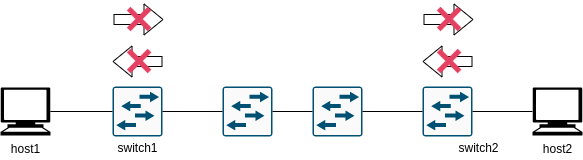
\includegraphics[width=0.7\linewidth]{img/example.png}
	\caption{Graphical representation of where the rules for denying the communications between two hosts are installed}
	\label{img:switch12_example}
\end{figure}

\noindent Thanks to this rules no other packets are allowed to pass from \textit{switch1} and \textit{switch2}. It is possible that some packets are in the network because they have passed the access switches before the intent expiry, in that case there are no problems because they are discarded in any case when they arrive in one of the two access switches. Those packets are a few (possibly 0) and so they doesn't affect the performance heavily, the alternative would be installing rules on each switch of the network in order to discard immediately these packets but this would be more costly.

\noindent When the rules are no longer valid for each packet arriving to \textit{switch1} or \textit{switch2} a packetIn is generated and thus the \textit{processPacketInMessage} method will check if that packet is allowed (an intent has been re-established) or not (the old intent has expired and no other intent have been established).

\noindent Notice that due to the fact that the rules installed in the switches are valid for a certain time, no intent can be established until that rules are no longer valid. In the default case the rules are valid for 5 seconds and so a new intent regarding one of the two hosts can be established 5 seconds after the expiry of the old intent. That time can be changed by the network manager through REST.

\noindent The last problems that need a solution is how we can know which is the identifier of \textit{switch1} and \textit{switch2}. When the timeout task (the task that will be performed when the intent expires) is created we pass to the constructor:
\begin{itemize}
	\item A reference to the object IntentForwarding, this is necessary in order to call the function who is in charge to install rules in the switches
	\item A reference to the object representing the intent associated to that timeout task. That object is \textbf{HostPair} and it is composed by:
	\begin{itemize}
		\item IPv4Address host1IP
		\item IOFSwitch sw1
		\item IPv4Address host2IP
		\item IOFSwitch sw2
		\item long timeout
	\end{itemize}
	\noindent That reference is necessary in order to retrieve the identifier of \textit{switch1} and \textit{switch2}. That identifiers are set when the first packetIn coming from the first switch encountered by the packet sent by an host is handled by the extended forwarding module i.e. IntentForwarding (for more on this see \ref{sec:Ipv4}).
\end{itemize}
\noindent Here we can see the code executed when we add an intent.

\begin{lstlisting}
	public boolean addNewIntent(HostPair newPair) {
		System.out.print("AddNewIntent Called\n");
		if(intentsDB.contains(newPair)) {
			log.info(" Intent already present in Intents List");
			return false;
		}
		
		long timeout = newPair.getTimeout();
		Timer timer = new Timer();
		TimerTask task = new TimeoutTask(newPair, this);
		timer.schedule(task, timeout);
		
		intentsDB.add(newPair);
		return true;
	}
\end{lstlisting}

\subsection{IPv4 Management}\label{sec:Ipv4}
\noindent When a packetIn regarding an IPv4 packet arrives the operations done are:
\begin{itemize}
	\item The intents database is searched:
	\begin{itemize}
		\item If exists an intent between the sender and the receiver (or viceversa) then
		\begin{itemize}
			\item If the sender is \textit{host1} and \textit{switch1} (in the object HostPair representing the intent) is null then \textit{switch1} is set equal to the identifier of the switch that has sent the packetIn that has triggered this execution of \textit{processPacketInMessage}. Same thing is done for \textit{host2} and \textit{switch2}. 
			\item Then the method of the super class (Forwarding.java) is invoked 
		\end{itemize} 
		\item Otherwise two rules are installed on the switch that sent the packetIn in order to deny the communication between the two hosts for a certain amount of time (as we have seen the default timeout is 5 seconds but that value can be customized through REST API).
	\end{itemize}
	\noindent Here a section of the method \textit{processPacketInMessage}. Notice that when setting the switch id, is the method \textit{setSw(IOFSwitch switch)} that checks if the switch is already set or not and set the switch only if it is not already set.
	\begin{lstlisting}
		HostPair hp = null;
		int hpIndex = intentsDB.indexOf(new HostPair(sourceIP, destinIP));
		if (hpIndex != -1)
		hp = intentsDB.get(hpIndex);
		
		if(hp != null && intentsDB.contains(hp)) {
			System.out.printf("allowing: %s - %s on switch %s \n",
			sourceIP.toString(), destinIP.toString(), sw.getId());	
			if(hp.getHost1IP().equals(sourceIP))
			hp.setSw1(sw);
			if(hp.getHost2IP().equals(sourceIP))
			hp.setSw2(sw);
			return super.processPacketInMessage(sw, pi, decision, cntx);	
		}
		denyRoute(sw, sourceIP, destinIP);
		denyRoute(sw, destinIP,sourceIP);
		return Command.CONTINUE;
	\end{lstlisting}
\end{itemize}


\subsection{ARP Management}
\noindent The ARP protocol is used to retrieve the layer 2 address of an host given its IP address. When an ARP packet arrives to a switch a packetIn is sent to the controller and so the processPacketInMessagge is invoked, the method understands that the packet that has triggered the packetIn is an ARP packet and so it must be handled differently.


\noindent The first operation done is checking if an intent between the sender and the receiver exists using their IPs. If an intent exists then the method of the super class is invoked otherwise the ARP packet is blocked.


\noindent The rules to avoid communication between the MACs addresses carried inside the ARP packet are installed only if that packet is an ARP response, in that case the target MAC address is not 00:00:00:00:00:00. In fact installing a rule that deny to forward an ARP messagge from a certain mac X to 00:00:00:00:00:00 means deny X to runs the ARP protocol because for each ARP request the target mac is 00:00:00:00:00:00 i.e. unspecified mac. Viceversa deny an ARP from 00:00:00:00:00:00 to any mac has no sense.	
	
	\section{REST API For Establishing An Intent}
	\noindent When the hostA wants to send an intent to make a connection with hostB it has to use the REST API. This API is provided by the classes: IntentWebRoutable, AddNewIntent, DelIntent and GetIntent; these classes use methods from IntentForwarding.
	
	\noindent When the REST API receives the intent, it establishes it inserting an entry in a dedicated data structure where it is indicated:
	\begin{itemize}
	\item The Source
	\item The Destination
	\item Intent Timeout
	\end{itemize}

	\noindent The possible API’s that we can use are:
        \begin{itemize}
        \item "/addNewIntent/json", that is used to insert new intent. This API gets from a JSON file two IPs (representing source and destination) and a timeout. This use the addNewIntent function of the IntentForwarding class that, first check if new intent is already presents, then in case it isn’t put it in intentDb that is an ArrayList of HostPair. Moreover, this function also set the timeout time of the pair.
        \item "/delIntent/json", that takes from a JSON file two IPs and a timeout and removes the intent corresponding to them. To do this, it use the delIntent function of IntentForwarding, that iterates the intentDB list and removes the intent with IPs passed in through JSON.
	\item "/getIntents/json", that is used to get all intents present in specific moment. It use the getIntents function of IntentForwarding that simply return intentDb.
        \end{itemize}

	
	
	\noindent Then the intent will be pushed in the network when the source host tries to send a packet to the destination host. When this happens a packetIn sending from the first switch that receives the packet will be sent to the controller and will be handled by the forwarding module seen in \ref{forwarding}
	
	\section{Responsiveness To Link Failures \& Topology Changes}
	To be responsiveness to topology changes we can exploit the ITopologyListener inteface. In fact in the Floodligh documentation for the TopologyService it is written: \textit{"All the information about the current topology is stored in an immutable data structure called the topology instance. If there is any change in the topology, a new instance is created and the topology changed notification message is called. If other modules want to listen for changes in topology they can implement the ITopologyListener interface."}\footnote{https://floodlight.atlassian.net/wiki/spaces/floodlightcontroller/pages/1343623/TopologyService+Dev}.
	
	\noindent Thus we can implement a class that implements ITopologyListener and that each time a topology change arrives it recompute the paths of intent involved in the topology change (i.e. the ones that has a link which doesn't work anymore). To do so we can use the TopologyInstance (updated before sending the notification message that the topology has changed) to understand which intent are involved in the topology change.
	
	\chapter{Testing}
	% !TeX spellcheck = en_US
\chapter{Testing}
\section*{Languages and Frameworks}
In order to test our system, we need to use a tool to create a \textit{virtual network} inside our machine: we used \texttt{mininet}\footnote{http://mininet.org/}, 
exploiting the \texttt{python2} APIs. To simulate input from an external application we also used a python2 library, called \texttt{requests}\footnote{https://docs.python-requests.org/en/latest/},
which is able to act like an HTTP client.\
Given that our developement environment is inside a virtual machine, we will keep the number of virtual devices relatively small, in order to not
overload the VM resources.

\section*{Scenario}
We want to simulate a typical data center scenario with a single LAN, implemented in a \textit{Spine-Leaf} topology. This configuration
is widely used thanks to its easy scalability and sufficient redundancy.
\begin{figure}[h]
    \centering
    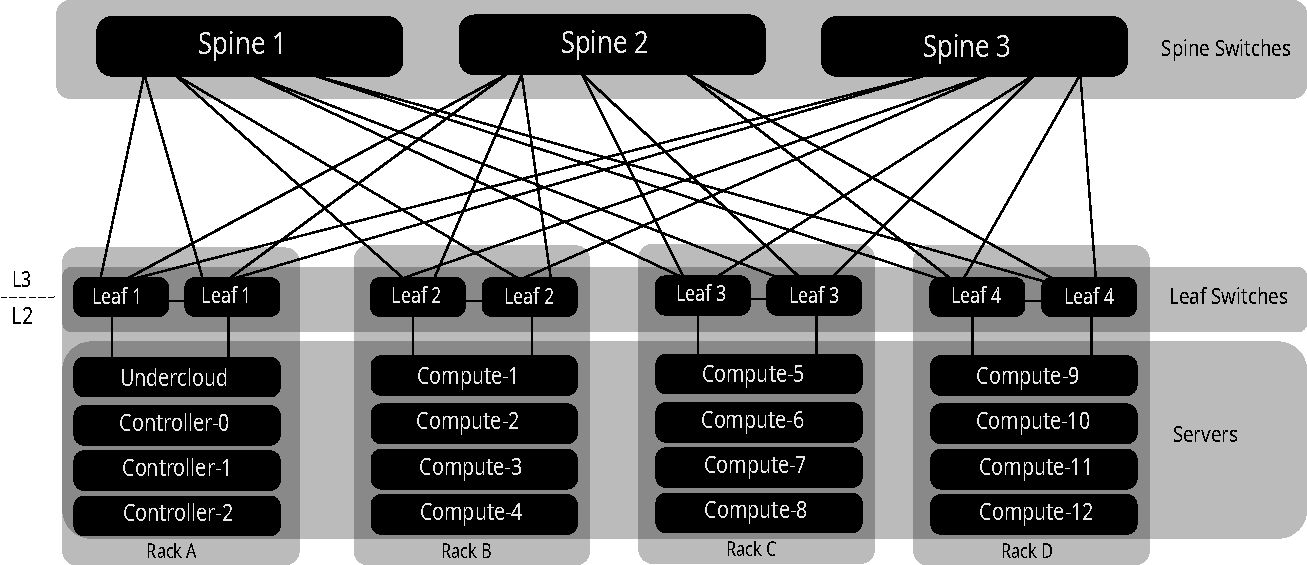
\includegraphics[width=0.90\textwidth]{img/spine_leaf.pdf}
    \caption{example of \textit{spine-leaf} topology}
\end{figure}

\section{Link Failure Test}
\noindent Using \texttt{mininet}, we can also simulate an episode of link failure, in order to test the system behaviour in this specific case. The system is able to recompute a functional path between two host and use it to forward packets.

\noindent In order to perform this test we use a spine leaf network with 2 spines and 3 leaf, each leaf has two hosts connected to it. The links of the network can be seen in figure \ref{img:links}

\begin{figure}[h]
	\centering
	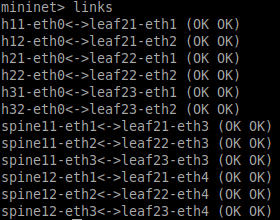
\includegraphics[width=0.50\textwidth]{img/links.png}
	\caption{Links of the spine leaf network}
	\label{img:links}
\end{figure}

\noindent To prove that the system is capable of handling a link failure we will establish an intent, use wireshark to sniff the traffic on the interfaces of the spines and see what happens when a link failure takes place and how the traffic is redirected.

\noindent The first thing to do is obviously to start the floodligh controller and the network\footnote{through the script scripts/start\_only\_spine\_topo.py}, then we establish an intent between the host11 (connected to leaf21) and the host21 (connected to leaf22). In order to check the connectivity we use wireshark on spine11-eth1 (the interface that connects leaf21 with spine11) and spine12-eth1 (the interface that connects leaf21 with spine12) and we perform a ping between the two hosts to see what happens on these interfaces.

\begin{figure}[h]
\centering
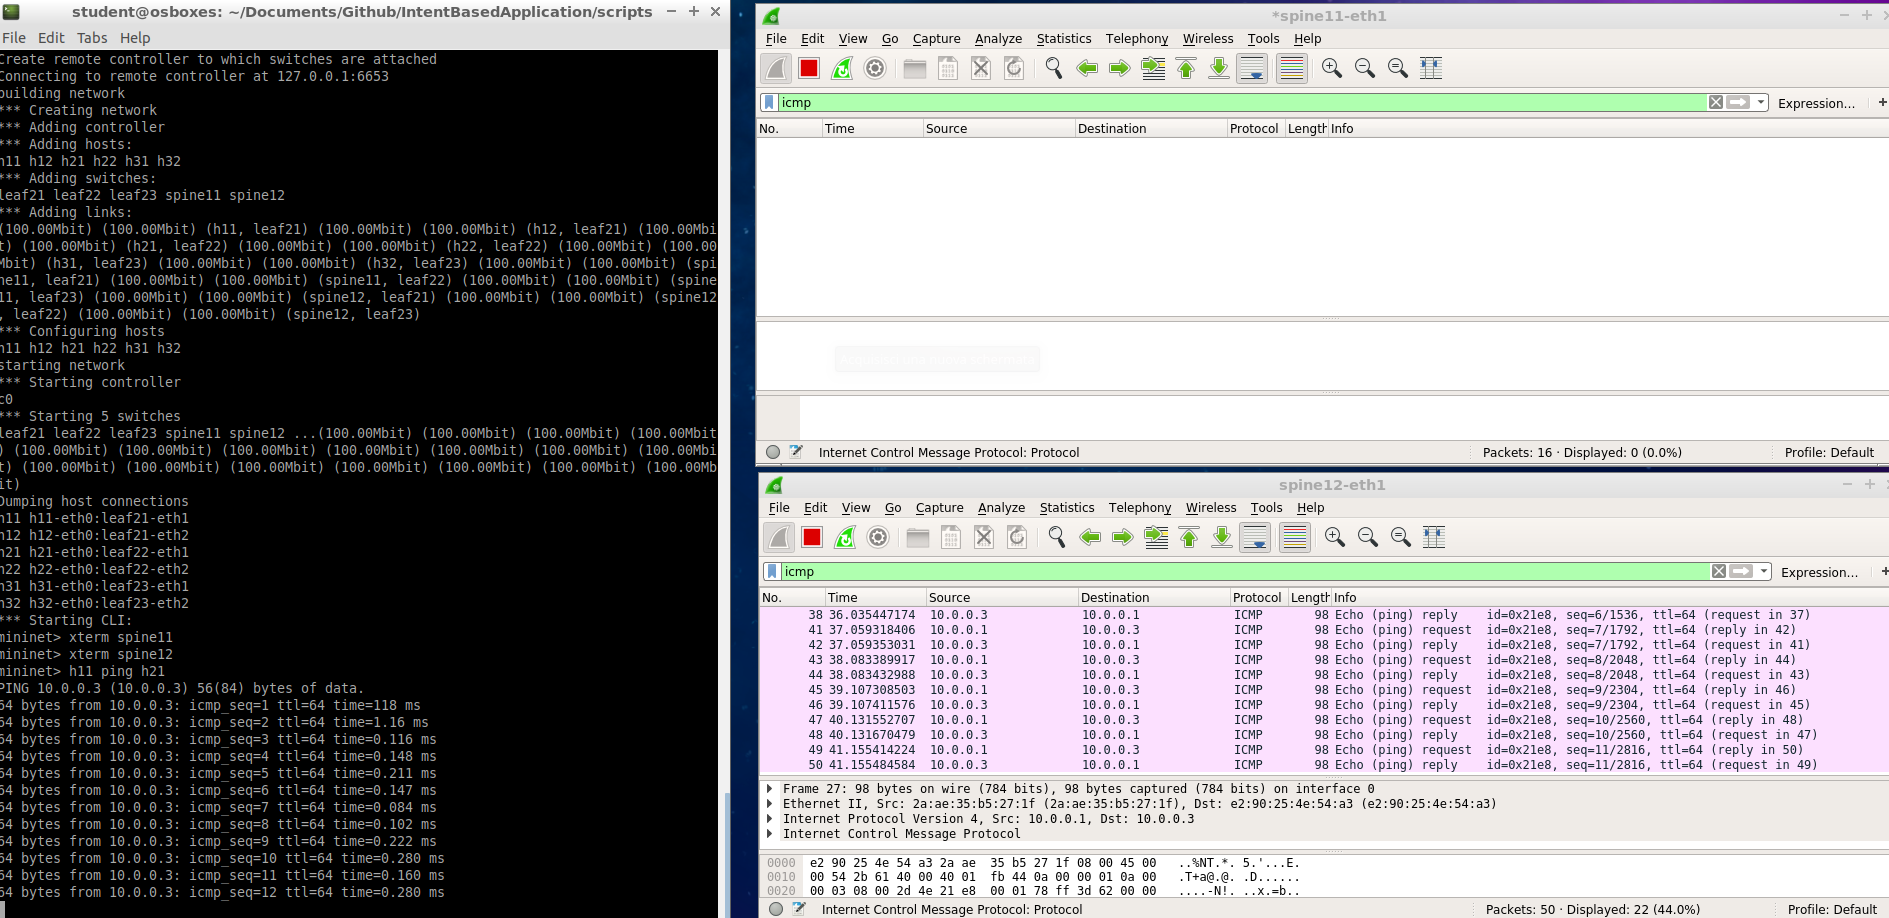
\includegraphics[width=1\textwidth]{img/ping1.png}
\caption{Ping between host11 and host21}
\label{img:ping1}
\end{figure}

\noindent As we can see in figure \ref{img:ping1} the ping is executed succesfully and the interface spine12-eth1 is used to forward the traffic. Now we put down the link between leaf21 and spine12, so the interface spine12-eth1 is now down (see figure \ref{img:linkdown}).

\begin{figure}[h]
	\centering
	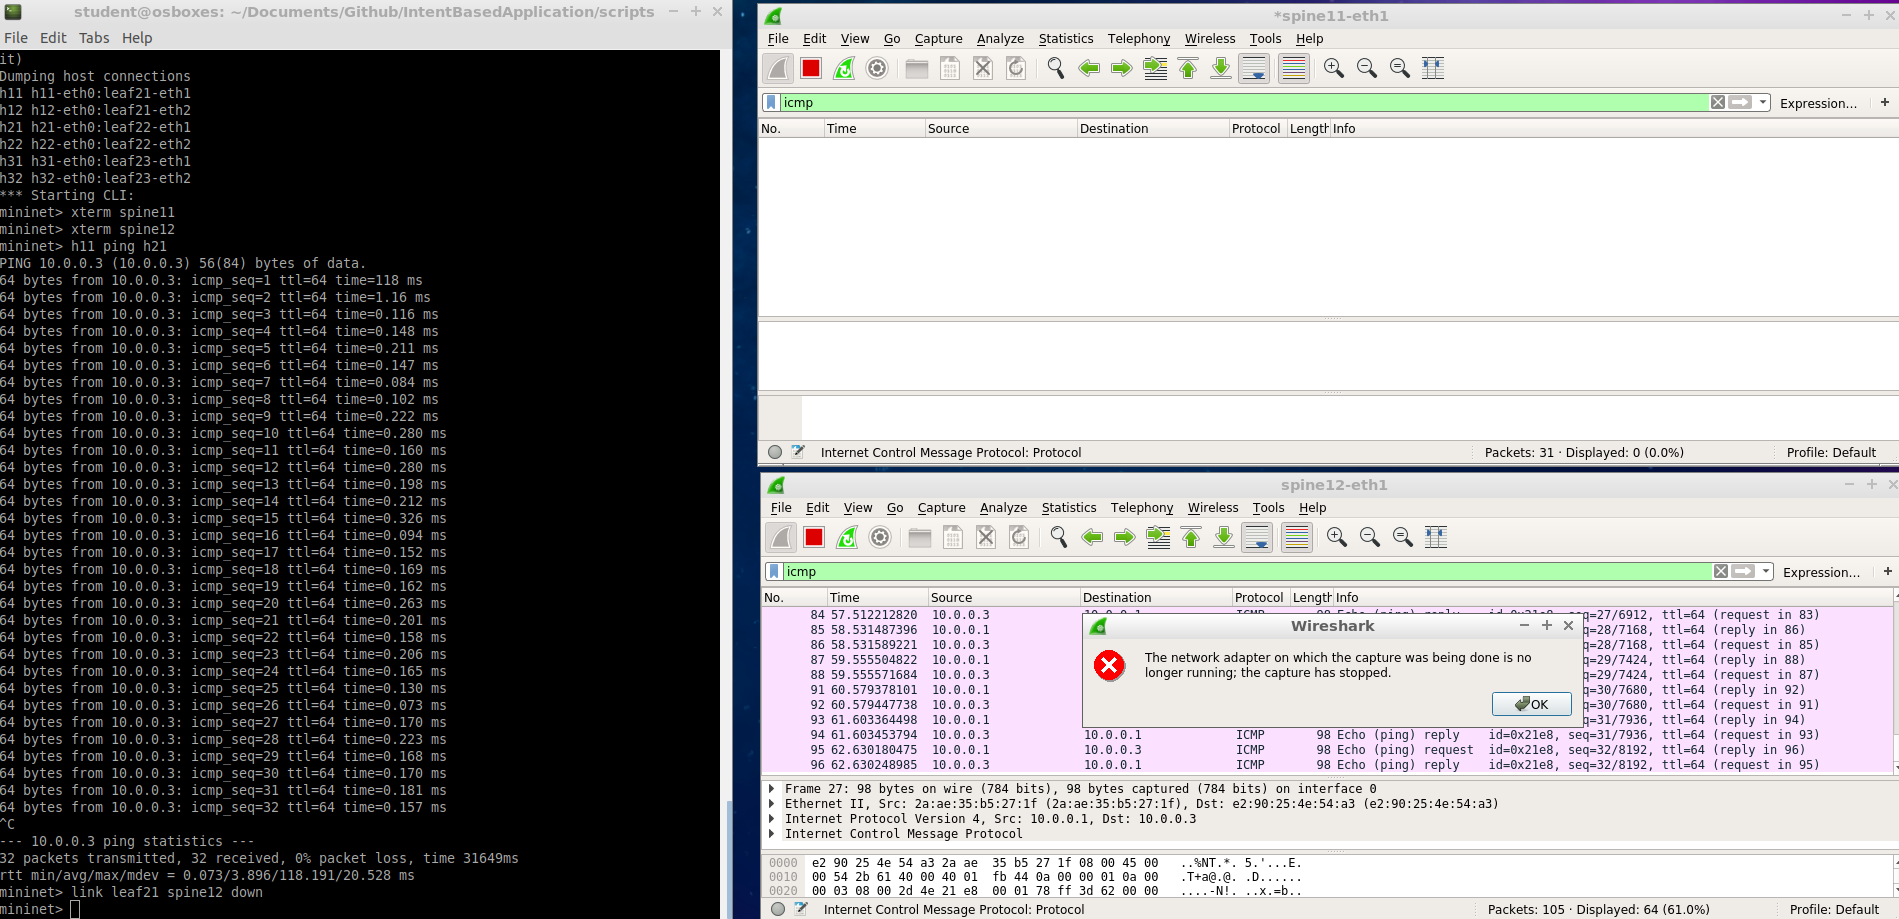
\includegraphics[width=1\textwidth]{img/linkdown.png}
	\caption{We put down the link between leaf21 and spine12}
	\label{img:linkdown}
\end{figure}

\noindent Then we perform another time the ping and we see that the interface spine11-eth1 is used to forward traffic (see figure \ref{img:failurehandler}).

\begin{figure}[h]
	\centering
	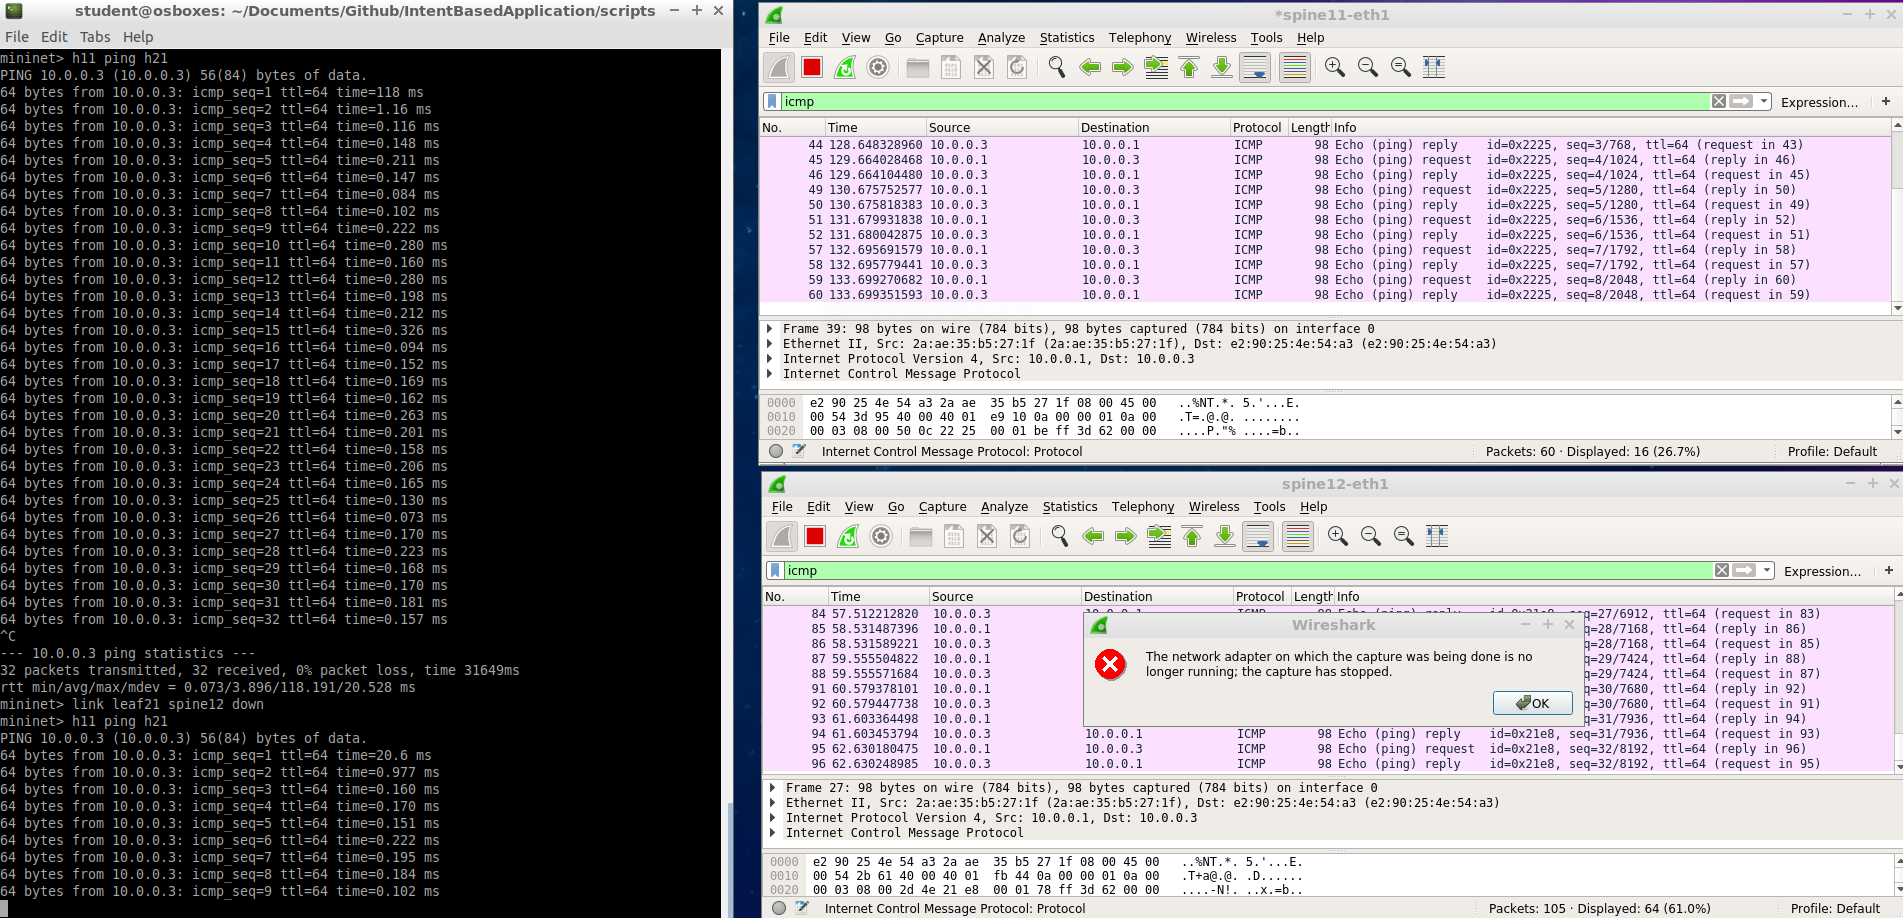
\includegraphics[width=1\textwidth]{img/failurehandler.png}
	\caption{Host11 now uses spine11-eth1 to perform the ping}
	\label{img:failurehandler}
\end{figure}

\noindent Thus we can state that at the beginning host11 used spine21 to communicate with host21 but when the link between leaf21 and spine21 failed (and so host11 cannot communicate anymore with spine21) host11 uses spine11 and so the intent continues to be valid. Hence the system is able to cope with a link failure.


\newpage
\section{Ping Latency}
In order to measure the network performance we will consider a fixed scenario with 2 spines, 3 leafs and 4 hosts for each leafs (i.e. 12 hosts in total);
for every host:
\begin{itemize}
    \item  we establish an intent with another random chosen one;
    \item  we start a ping session, measuring the \texttt{round trip time} of each packet
    \item  the session end when 10 ping are successfully exchanged, or the last timeout elapses
\end{itemize} 
\begin{figure}[h]
    \centering
    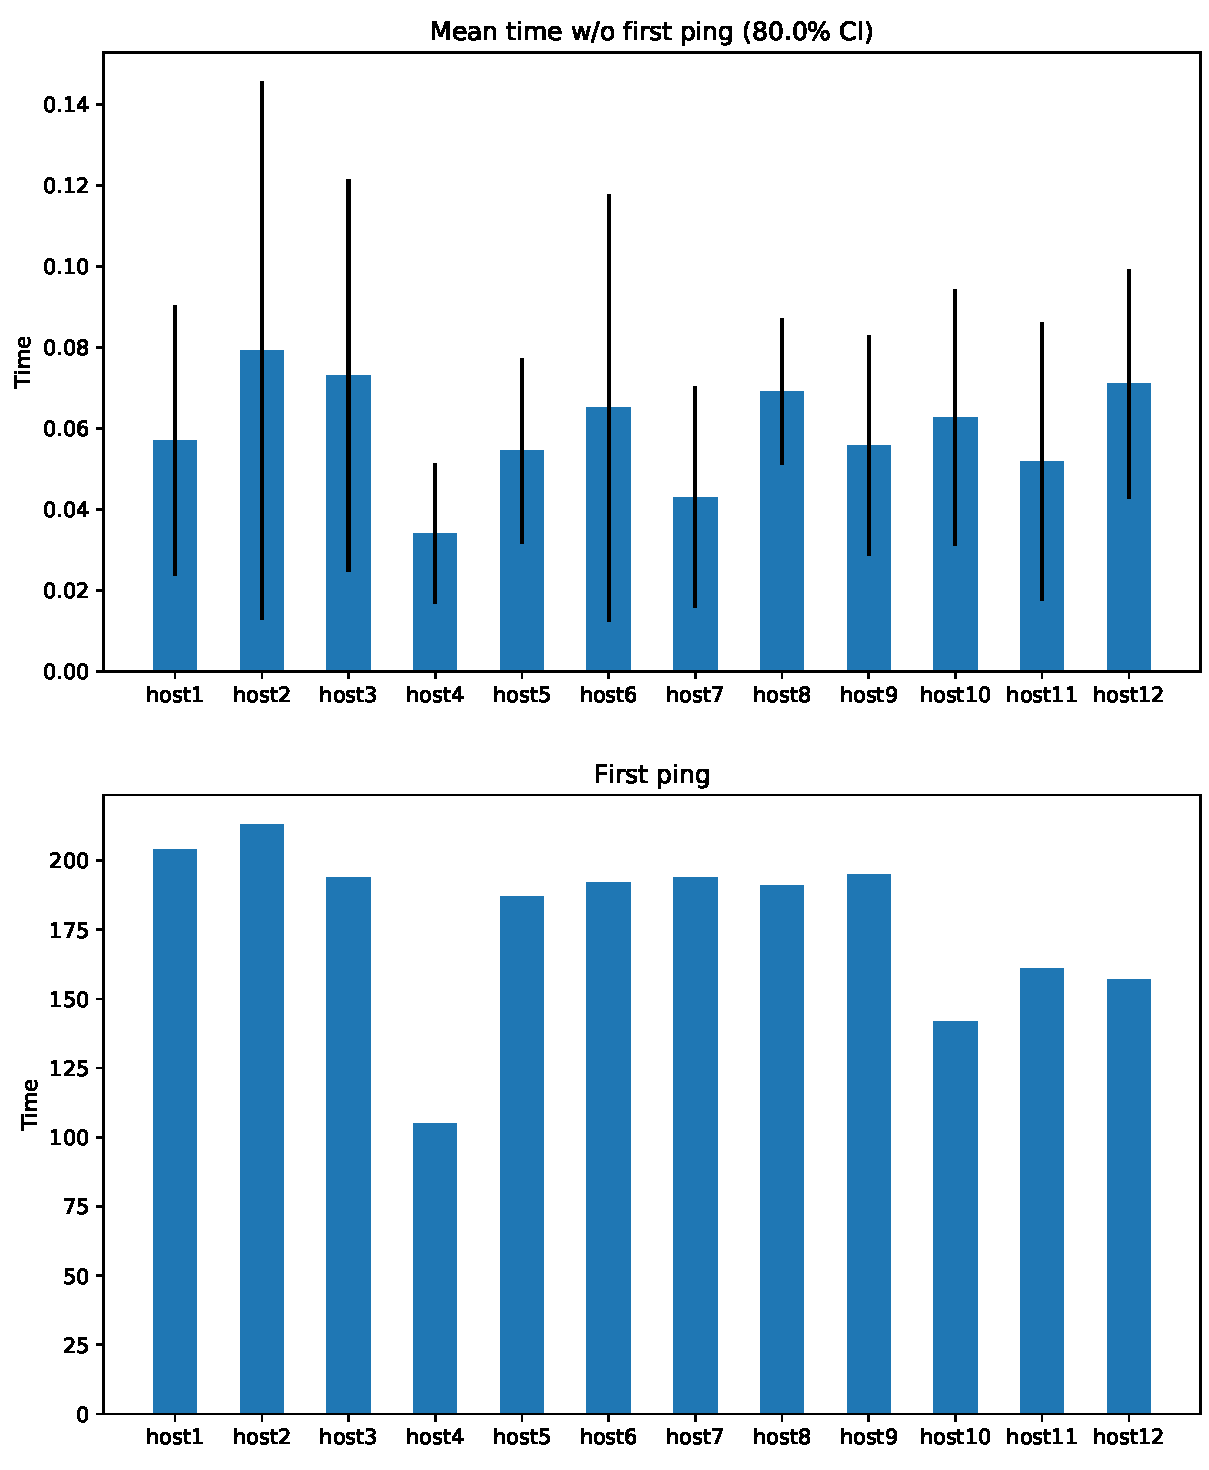
\includegraphics[width=.92\textwidth]{img/mean_ping_time.pdf}
    \caption{Ping times with 12 hosts}
    \label{img:perf1}
\end{figure}
First of all we monitor the number of \texttt{DESTINATION HOST UNREACHABLE} and \texttt{DUPLICATE}, those 2 parameters are equal to 0, confirming the correct
behaviour of the network.
The performance results (see figure \ref{img:perf1}) are consistent with our expectation:
\begin{itemize}
    \item the first ping is significantly slower than the others, because it is processed by the controller, triggering the route establishment;
    \item subsequent pings are very fast (<1 ms), because they don't have to traverse "real" network cables and because they are processed by the virtual switches and not by the controller.
\end{itemize}
\newpage
\begin{figure}[h]
    \centering
    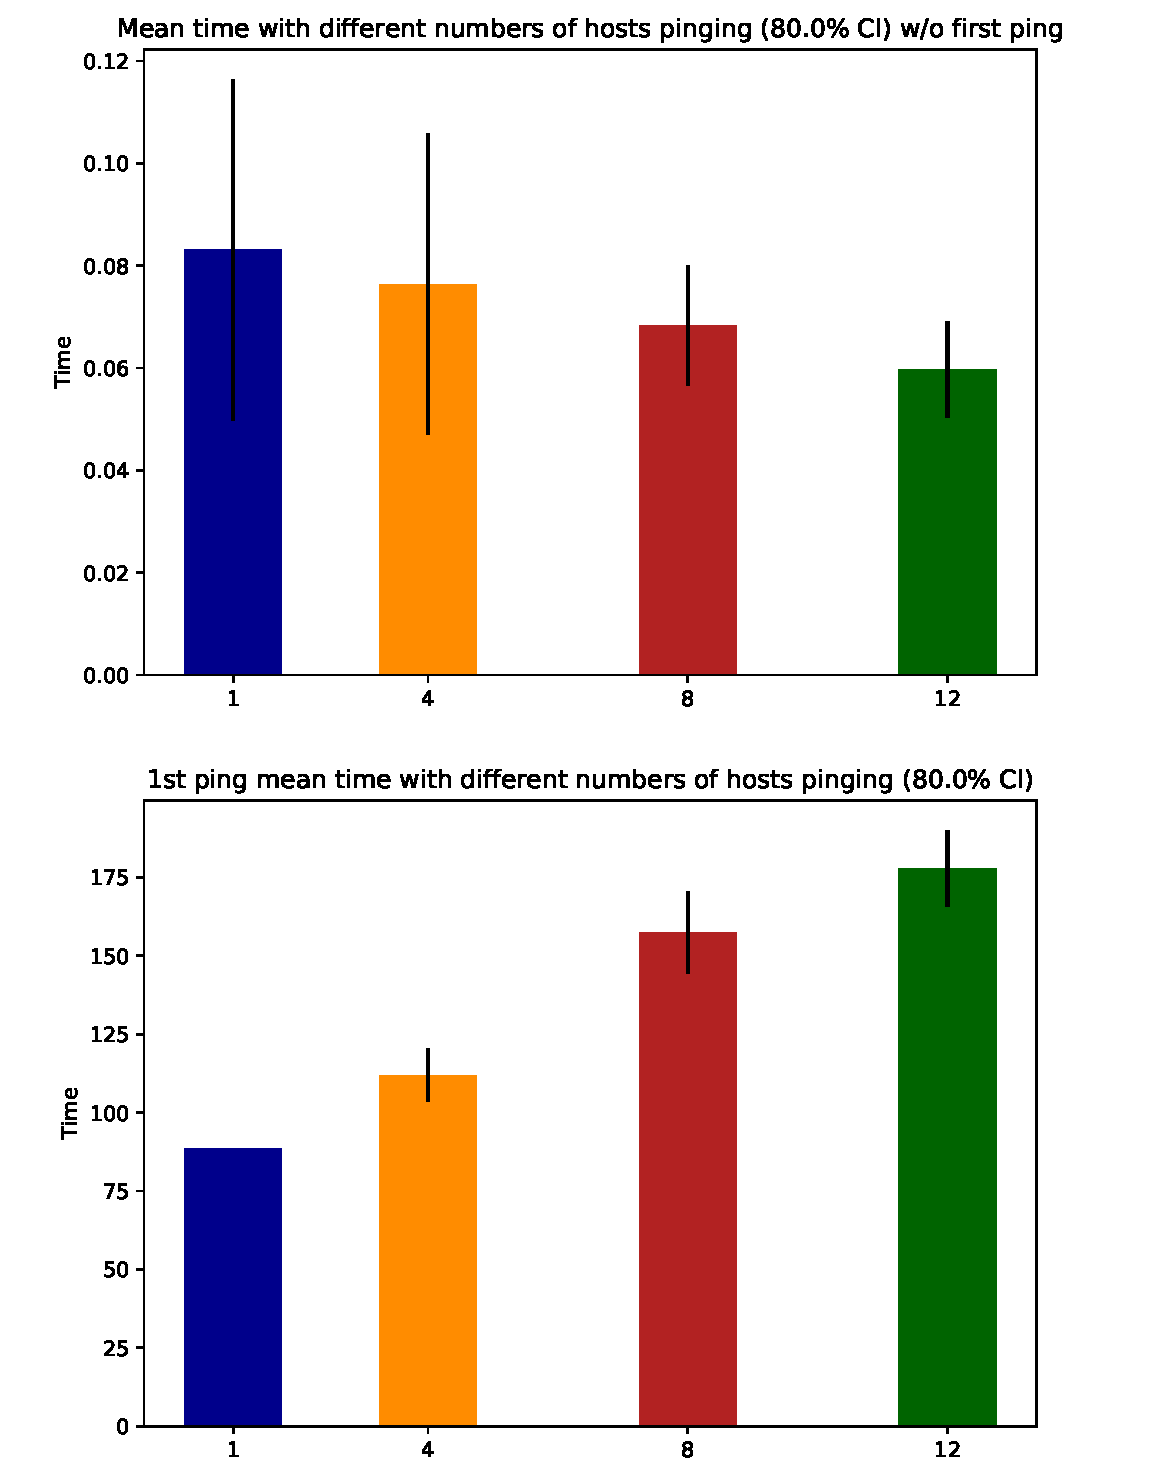
\includegraphics[width=.94\textwidth]{img/increasing_ping_time.pdf}
    \caption{Ping times with different loads}
    \label{img:perf2}
\end{figure}
\noindent We also tried to evaluate the elasticity of the network with increasing load of traffic (i.e. increasing number of host pinging at the same time) and the results of this tests can be seen in figure \ref{img:perf2}.\\
The time needed for the first ping to complete tends to increase with the amount of traffic meanwhile the time for the others pings remains pretty stable
(mind the confidence intervals). This is expected because route establishment is done by the controller in a centralized way (the requests will queue up);
once the route is established, switches will handle the traffic in a distributed manner, leading to optimal forwarding of traffic.
\end{document}
